\begin{frame}

\frametitle{OpenGL}

OpenGL is a graphics API (similar in scope to Direct3D) that allows to use the
graphics card to draw 2D and 3D vector graphics.

\begin{itemize}
    \item{1992 - OpenGL is first released}
    \item{2004 - OpenGL 2.0 is released. Adds support for programmable pipeline (shaders).}
    \item{2010 - OpenGL 4.0 is released. Adds support for geometry shader (tesselation).}
\end{itemize}

\begin{center}
    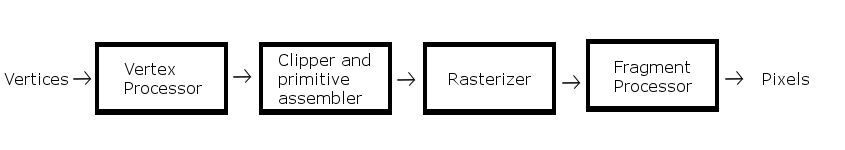
\includegraphics[width=\textwidth]{images/pipeline.png}
\end{center}

\end{frame}

\begin{frame}[fragile]

\frametitle{Old method for drawing}

\begin{center}
\begin{lstlisting}
glColor3f(1.0f, 0.0f, 0.0f);
glBegin(GL_QUADS);
    glVertex2f(-0.25f, 0.25f);
    glVertex2f(-0.5f, -0.25f);
    glVertex2f(0.5f, -0.25f);
    glVertex2f(0.25f, 0.25f);
glEnd();
\end{lstlisting}
\end{center}

Moreover the API had to support many features, for example textures coordinates,
lighting, shadows, coordinate transformation and perspective matrices.

\vspace{5mm}

This results in a complex API and lack of flexibility.

\end{frame}

\begin{frame}[fragile]

\frametitle{Modern approach}



\end{frame}


\begin{frame}[fragile]

\frametitle{OpenGL state machine}

Since the rendering of the 3D scene is a very complex task, OpenGL uses
the concept of state machine to simplify the API interface (avoid function
with too many arguments).

\begin{center}
\begin{lstlisting}
// Tell OpenGL which array contains the data
glBindBuffer(GL_ARRAY_BUFFER, vbo);
// Specify how the data for position can be accessed
glVertexAttribPointer(0, size, GL_FLOAT, GL_FALSE, 0, 0);
// Enable the attribute
glEnableVertexAttribArray(0); // location = 0

// Draw
glDrawArrays(type, 0, vertex_num);
\end{lstlisting}
\end{center}

\end{frame}

\begin{frame}[fragile]

\frametitle{OpenGL VBOs}

VBO (Vertex Buffer Object) - is an array of data in the GPU memory for storing vertices.

\end{frame}

\begin{frame}[fragile]

\frametitle{OpenGL Textures}

Texture - is an image that is mapped to vertices.

\begin{center}
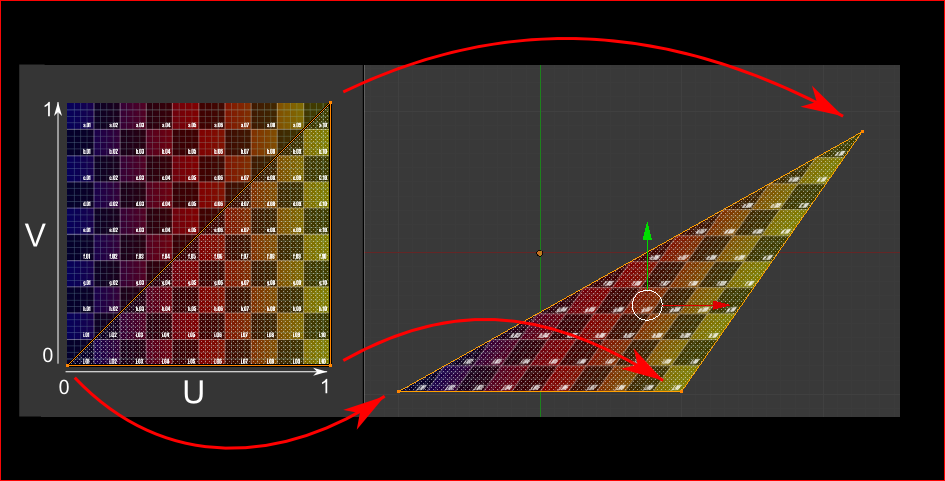
\includegraphics[width=\textwidth]{images/uv.png}
\end{center}

\end{frame}

% Brief into to opengl
% Intro
% Advantages - Disadvantages
% Execution model
% Registering and Mapping
% State machine
% Arrays and Textures
% Shaders
% Drawing
% Show code
